
%(BEGIN_QUESTION)
% Copyright 2010, Tony R. Kuphaldt, released under the Creative Commons Attribution License (v 1.0)
% This means you may do almost anything with this work of mine, so long as you give me proper credit

PT-56 measures gas pressure inside a chemical reactor vessel over a range of 0 to 25 PSI, through a remote seal:

$$\includegraphics[width=15.5cm]{i03557x01.eps}$$

The pressure transmitter is presently mounted 14 feet below the remote seal, with a fill fluid density of 66.8 lb/ft$^{3}$.  A decision is made to replace the existing remote seal transmitter with a new remote seal transmitter having a different fill fluid with a density of 78.2 lb/ft$^{3}$, because the new (denser) fill fluid is safer than the old fluid from the perspective of chemical reactivity.  Your task is to determine how to reconfigure the new transmitter to work properly in this system.  Based on this information, answer the following questions:

\vskip 10pt

For new fill fluid type: LRV = \underbar{\hskip 50pt} PSI \hskip 30pt  URV = \underbar{\hskip 50pt} PSI

\vskip 10pt

Does the change in fill fluid type necessitate a different isolation diaphragm size, or will the old size work just fine?

\vskip 10pt

Does the change in fill fluids necessitate a change in controller action from direct to reverse, or vice-versa?

\vskip 10pt

Assuming an air-to-open PV-56 control valve, does PIC-56 need to be {\it direct} or {\it reverse} acting?

\underbar{file i03557}
%(END_QUESTION)





%(BEGIN_ANSWER)

\noindent
(2 points each)

LRV = \underbar{\bf 7.60} PSI \hskip 30pt  URV = \underbar{\bf 32.60} PSI

\vskip 10pt

\noindent
(2 points)

The old isolation diaphragm size will work just fine.

\vskip 10pt

\noindent
(2 points)

The change in fill fluid type does {\bf not} necessitate any change in controller action.

\vskip 10pt

\noindent
(2 points)

Assuming an air-to-open PV-56 control valve, PIC-56 needs to be {\bf reverse} acting.


%(END_ANSWER)





%(BEGIN_NOTES)

{\bf This question is intended for exams only and not worksheets!}.

%(END_NOTES)


